\chapter{User Interface and Experience Design}

This chapter outlines the essential steps that define the structure of the application and primarily focus on shaping its frontend. These steps are crucial in determining the tools and methods required to meet the application's demands before any coding begins. Among these steps are the creation of mockups, which establishes the layout and structure of the application's screens; the selection of design elements, which contribute to the aesthetic and user-friendly aspects of the interface; and finally, the searching of inspiration for screens and components, that align also with the final design of the mockups. These components guide the development of the application's necessary features and layout, ensuring both functionality and visual appeal.

\section{Mockups}

In this section, we design the mockups based on the requirements gathered in the previous chapter, ensuring that each design element aligns with the core functionalities of the application. For this purpose, I use \textbf{Figma}, a collaborative design tool widely used for creating user interfaces and prototypes. Figma allows for real-time collaboration and provides a streamlined interface for designing, testing, and refining mockups. Once the initial designs are complete, the mockups are evaluated to assess their usability, functionality, and alignment with user needs. Based on this evaluation, any necessary adjustments are made, leading to the final design of the mockups that are implemented in the application.

\subsection{Initial Design}

\noindent \textbf{Welcome Screen (Before Connection) [\ref{fig:welcome_1}]} \\
This is the initial screen that the user encounters when opening the application for the first time. It provides two button options:

\begin{itemize}
    \item \textbf{Login}: When pressed, the user is navigated to the ``Login screen'', to login with an existing account.
    \item \textbf{Register}: When pressed, the user is navigated to the ``Registration screen'', where new users can create an account.
\end{itemize}

\noindent This screen is going to be designed to be simple and straightforward, ensuring ease of access for new and old users.

\vspace{5mm}

\noindent \textbf{Welcome Screen (After Connection) [\ref{fig:welcome_2}]} \\
If the user has logged in the device a previous time, a geeting is shown with a personalized message, ``Welcome back, \{Name\}''. Below this greeting, the user is provided with the question ``How are you feeling today?'' and an Emoji Selector, which leads them to log their daily mood using emojis. On the other hand, if the logged-in account is incorrect (the correct name is shown), users can select one of the following buttons:
\begin{itemize}
    \item \textbf{Login}: When pressed, the user is navigated to the ``Login screen'', to login with a different account.
    \item \textbf{Register}: When pressed, the user is navigated to the ``Registration screen'', to create a new account, if they don't have one already.
\end{itemize}

\vspace{5mm}

\noindent \textbf{Registration Screen [\ref{fig:registration}]} \\
This screen allows new users to create an account. Users must provide their:
\begin{itemize}
    \item First Name
    \item Last Name
    \item Email
    \item Password
    \item Password Confirmation
\end{itemize}

\noindent There’s also a prompt for users who may already have an account, directing them back to the ``Login screen'' with the link ``Already having an account?''.

\vspace{5mm}

\noindent \textbf{Login Screen [\ref{fig:login}]} \\
Users with an existing account can sign in by providing:
\begin{itemize}
    \item Email
    \item Password
\end{itemize}

\noindent For users who do not yet have an account, a link is provided, ``Not having an account?''. This takes them to the ``Registration screen''.

\vspace{5mm}

\noindent \textbf{Profile Screen [\ref{fig:profile}]} \\
This screen displays the user's profile information and can be accessed when pressing the avatar icon on the top right corner of some screens. The profile information consists of:

\begin{itemize}
    \item Full Name
    \item Email
\end{itemize}

\noindent Users can choose to edit their profile by clicking the ``Edit Profile'' button. They are also given the option to Log Out.

\vspace{5mm}

\noindent \textbf{Edit Profile Screen [\ref{fig:edit_profile}]} \\
In this screen, users can modify the profile information by pressing the ``Save Changes'' button shown in the top right corner of the ``Profile Screen''. The information contains:
\begin{itemize}
    \item First Name
    \item Last Name
    \item Email
    \item Old Password
    \item New Password
\end{itemize}

\noindent Upon making changes, users can save their updates by clicking the ``Save Changes'' button.

\vspace{5mm}

\noindent \textbf{Main Menu Screen [\ref{fig:main_menu}]} \\
This is the central navigation hub of the application, that the user enters after logging in. It offers access to four key features:
\begin{itemize}
    \item \textbf{Daily Survey}: Users can log their daily mood.
    \item \textbf{Previous Surveys}: Access previous mood logs and review past entries.
    \item \textbf{General Stats}: View statistics of mood data over time.
    \item \textbf{Journal}: Allows users to write personal reflections or entries.
\end{itemize}

\vspace{5mm}

\noindent \textbf{Today's Survey Screen [\ref{fig:todays_survey}]} \\
This screen is accessed when the user selects the ``Daily Survey'' option from the ``Main Menu Screen''. It presents one of the question of the daily survey. In complete, the daily survey consists of 4-5 screens like the figure image, each displaying:
\begin{itemize}
    \item \textbf{Date}: The date that the survey was posted.
    \item \textbf{Question Number}: The number of the question that the user is currently.
    \item \textbf{Question Text}: The original question presented during the survey.
    \item \textbf{Answer Options}: The answer options of the questionnaire, in our case ``Not True'', ``Sometimes'', ``True''.
    \item \textbf{Comment Section}: The section where the user can leave a comment for explaining better the answer, thus their mood.
\end{itemize}
\noindent Also in the bottom section of the screen there are some action buttons, that depending on if the user is on the last question or not, it shows the ``Submit'' or the ``Continue'' button respactively.

\vspace{5mm}

\noindent \textbf{Survey Menu Screen [\ref{fig:survey_menu}]} \\
This screen is displayed when the user selects the ``Previous Surveys'' option from the ``Main Menu Screen''. The screen is going to be scrollable and contains:
\begin{itemize}
    \item \textbf{Date}: The date that the survey was posted.
    \item \textbf{Questions}: The questions referring to this specific survey.
\end{itemize}
\noindent Each question consists of multiple questions, each of them consisting of:
\begin{itemize}
    \item \textbf{Question text}: Displays the original question presented during the survey.
    \item \textbf{Answer section}: Shows the user's previously selected answer or response.
    \item \textbf{Comment section}: Displays any additional comments the user wrote to add some context to their answer.
\end{itemize}

\noindent Users can navigate between surveys by clicking Previous or Next, allowing them to review their mood data over different days or weeks.

\vspace{5mm}

\noindent \textbf{Positive Confirmation Screen [\ref{fig:positive_confirmation}]} \\
This screen is displayed after the user completes and submits the daily survey. It provides feedback to the user, confirming the successful submission. The screen is simple and includes:
\begin{itemize}
    \item \textbf{Confirmation Message}: A message that informs the user they have successfully completed the survey, often accompanied by a visual indicator or icon (e.g., a checkmark).
\end{itemize}

\vspace{5mm}

\noindent \textbf{Statistics Screen [\ref{fig:statistics}]} \\
This screen is accessible from the ``Main Menu Screen'' by selecting the ``General Stats'' option. It allows the user to visualize their mood data over time. The screen includes:
\begin{itemize}
    \item \textbf{Calendar}: A visual calendar displaying the dates on which mood data was logged. Days with data entries are typically highlighted, giving the user a quick overview of their activity.
    \item \textbf{Graph}: A graphical representation of mood trends, showing how the user's mood has changed over time. This may include line graphs or bar charts for clarity.
\end{itemize}

\vspace{5mm}

\noindent \textbf{Journal Screen [\ref{fig:journal}]} \\
This screen is accessed from the ``Main Menu Screen'' by selecting the ``Journal'' option. It provides a space for the user to write personal reflections or additional details about their mood or experiences. The Journal Screen features:
\begin{itemize}
    \item \textbf{Date and Time}: A timestamp indicating when the journal entry is being written.
    \item \textbf{Text Field}: A large input field where the user can write their journal entry, sharing thoughts, feelings, or specific details about their mood.
\end{itemize}
\noindent Users can navigate between journal entries using the ``Previous'' and ``Next'' buttons, allowing them to review past entries. After completing a new entry, users can save it by clicking the ``Submit'' button.

\vspace{5mm}

\FloatBarrier
\begin{figure}[htbp]
    \centering
    \subfloat[Welcome Screen (before connection)]{\fbox{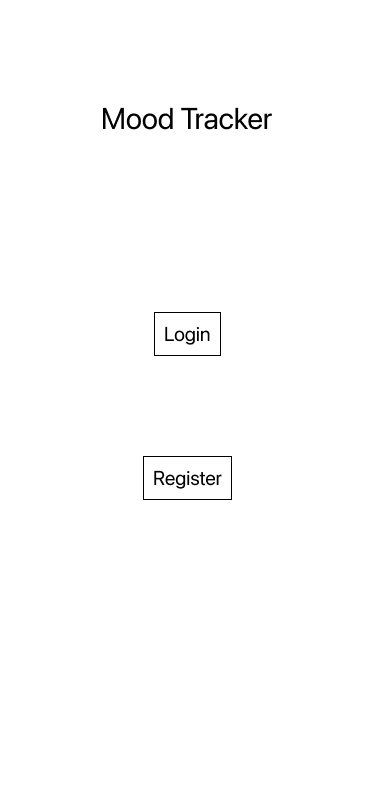
\includegraphics[width=0.3\linewidth]{figures/old-mockups/Welcoming.png}}\label{fig:welcome_1}}
    \hfill
    \subfloat[Welcome Screen (after connection)]{\fbox{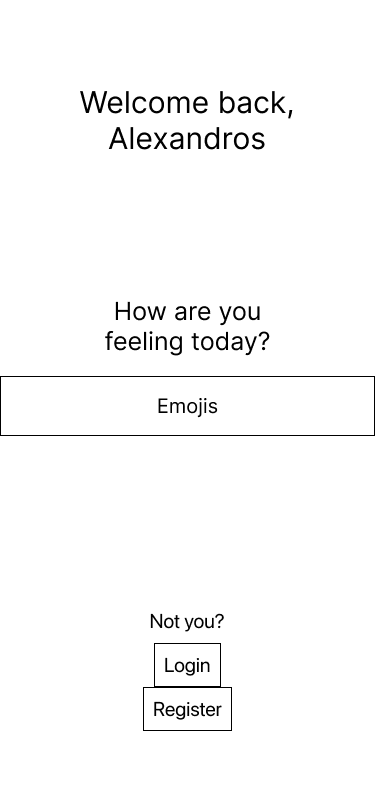
\includegraphics[width=0.3\linewidth]{figures/old-mockups/Welcoming-2.png}}\label{fig:welcome_2}}
    \hfill
    \subfloat[Registration Screen]{\fbox{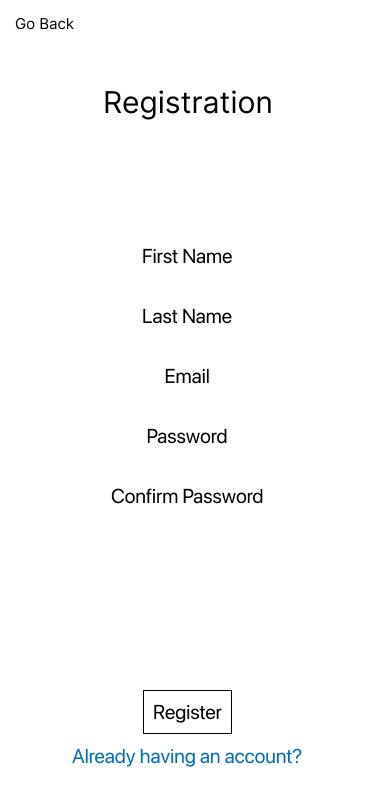
\includegraphics[width=0.3\linewidth]{figures/old-mockups/Registration.png}}\label{fig:registration}}
\end{figure}

\begin{figure}[htbp]\ContinuedFloat
    \centering
    \subfloat[Login Screen]{\fbox{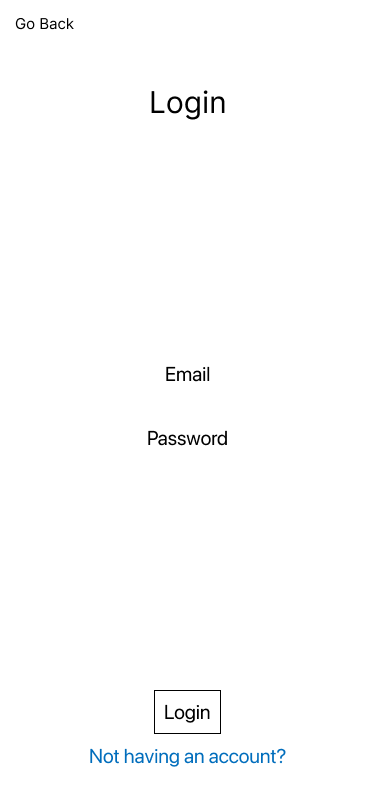
\includegraphics[width=0.3\linewidth]{figures/old-mockups/Login.png}}\label{fig:login}}
    \hfill
    \subfloat[Profile Screen]{\fbox{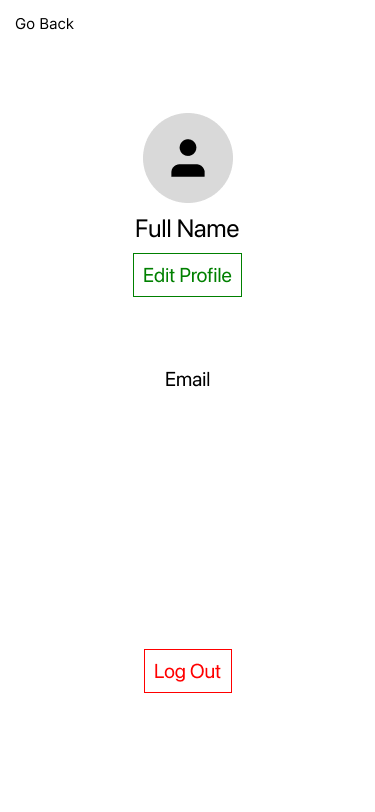
\includegraphics[width=0.3\linewidth]{figures/old-mockups/Profile.png}}\label{fig:profile}}
    \hfill
    \subfloat[Edit Profile Screen]{\fbox{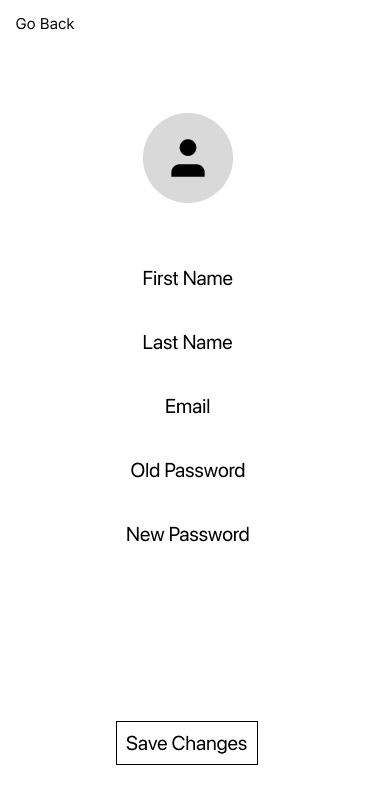
\includegraphics[width=0.3\linewidth]{figures/old-mockups/Edit Profile.png}}\label{fig:edit_profile}}
\end{figure}

\begin{figure}[htbp]\ContinuedFloat
    \centering
    \subfloat[Main Menu Screen]{\fbox{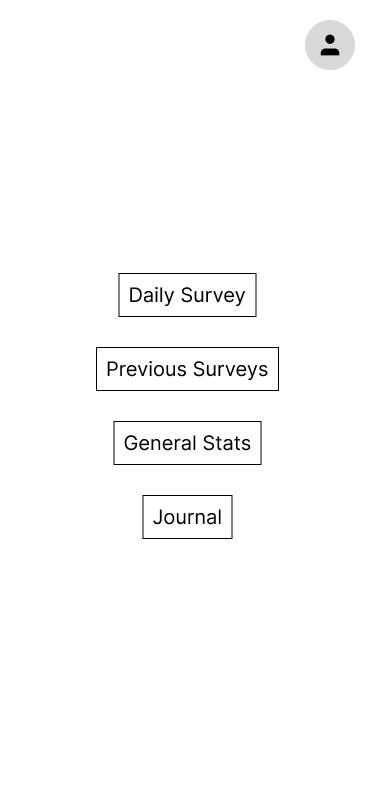
\includegraphics[width=0.3\linewidth]{figures/old-mockups/Main Page.png}}\label{fig:main_menu}}
    \hfill
    \subfloat[Today's Survey (All Screens)]{\fbox{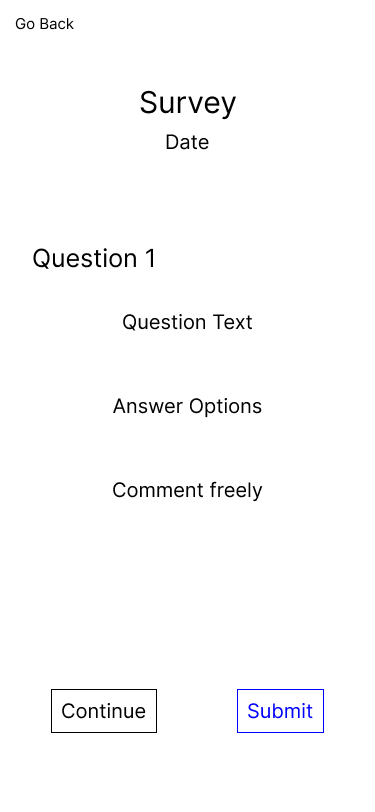
\includegraphics[width=0.3\linewidth]{figures/old-mockups/Today's Survey (All Pages).png}}\label{fig:todays_survey}}
    \hfill
    \subfloat[Survey Menu Screen]{\fbox{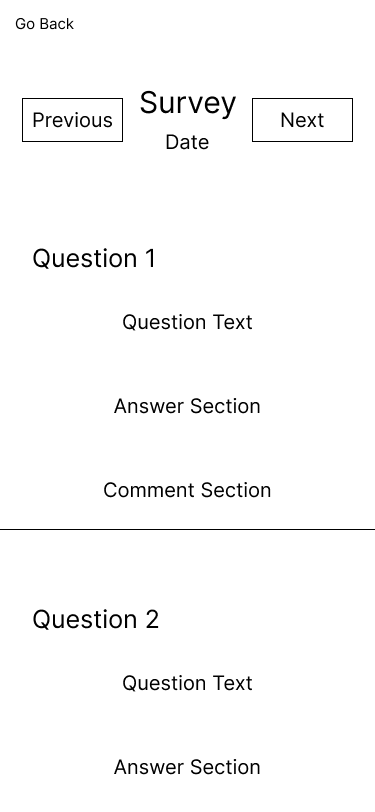
\includegraphics[width=0.3\linewidth]{figures/old-mockups/Survey Menu.png}}\label{fig:survey_menu}}
\end{figure}

\begin{figure}[htbp]\ContinuedFloat
    \centering
    \subfloat[Positive Confirmation Screen]{\fbox{
\includegraphics[width=0.3\linewidth]{figures/old-mockups/Positive Confirmation.png}}\label{fig:positive_confirmation}}
    \hfill
    \subfloat[Statistics Screen]{\fbox{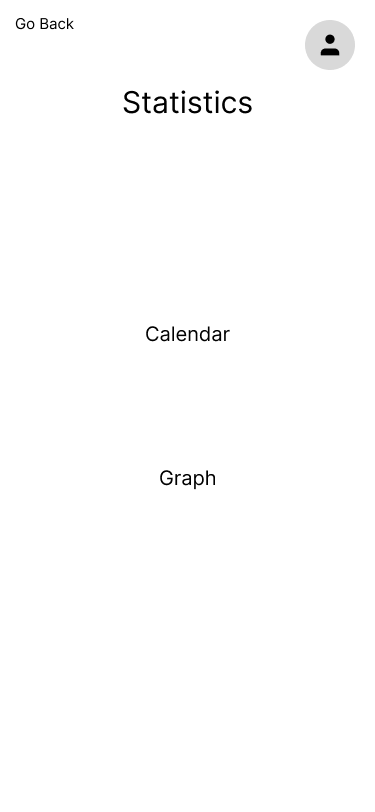
\includegraphics[width=0.3\linewidth]{figures/old-mockups/Statistics.png}}\label{fig:statistics}}
    \hfill
    \subfloat[Journal Screen]{\fbox{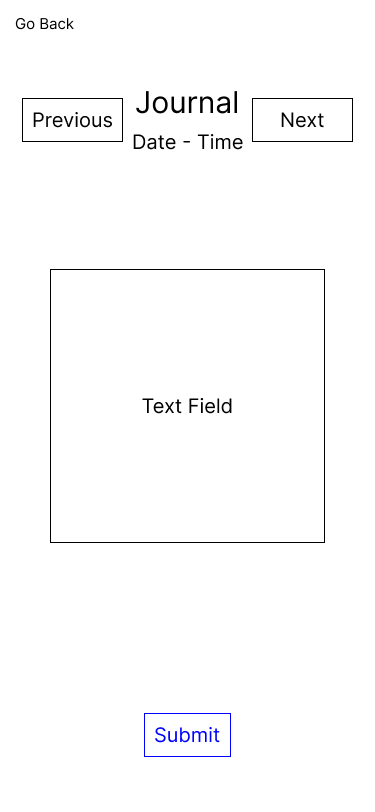
\includegraphics[width=0.3\linewidth]{figures/old-mockups/Journal.png}}\label{fig:journal}}
    \caption{User Flow Screens}
    \label{fig:user_flow_screens}
\end{figure}
\FloatBarrier

\subsection{Evaluation}

During the design process, we supervisor revisited the initial mockups with the objective of simplifying the user interface and focusing on only the most essential features of the application. After careful reflection on the functionality of each screen and discussions with my supervisor, it became clear that some screens could be reduced or merged to create a more streamlined and efficient user experience. The goal was to minimize unnecessary complexity and ensure that the app remained as simple and focused as possible, aligning with the overall aim of the thesis.\vspace{5mm} \\
Key modifications include reducing the number of screens and removing non-essential elements, such as the journal feature, which was identified as adding too much information and detracting from the core functionality of the app. The resulting design emphasizes a minimalist and straightforward approach, prioritizing clarity and simplicity over unnecessary features, ensuring that the app serves its primary purpose effectively.\vspace{5mm} \\
Firstly, the ``Welcome Screen'' was simplified into a single screen that greets the user daily, whether they log in or register. In the updated design, the ``Welcome Screen'' prompts the user to select a mood for the day, called the ``Welcome Mood''. This update creates a more engaging daily interaction with the app, encouraging users to immediately log their mood, which is then reflected in the statistics.\vspace{5mm} \\
In terms of navigation, the ``Main Menu Screen'' has undergone several improvements. Instead of a button for the ``Questionnaires Screen'', this option is part of a navigation bar, making it easier to access without cluttering the main screen. The ``Daily Message'', either a quote or advice, is more personalized to provide users with a motivational or reflective element every day. Additionally, the ``Data Projection'' feature shows a smaller version of the overall statistics, giving users a quick snapshot of their mood trends and questionnaire results.\vspace{5mm} \\
The ``Statistics Screens'' were refined to better reflect the user's mood and questionnaire data. The ``Calendar Screen'' projects the ``Welcome Moods'' that the user logs each day, providing a clear and visual history of daily moods. The ``Graph Screen'' is responsible for projecting the results from the questionnaires, allowing users to track how their answers have evolved over time.\vspace{5mm} \\
In the ``Survey Screens'', some adjustments were made to improve clarity and flow. In the updated design of the ``Today's Survey Screen'', the user navigates through the survey with a ``Continue'' button for intermediate questions and a ``Submit'' button for the final question, because it submits the whole survey. Similarly, the ``Previous Survey Screen'' maintains the same structure as the updated ``Today's Survey Screen'' but has additional navigation options. These include an ``Exit'' button, allowing the user to leave the survey, and a ``Continue'' button to navigate through all previously answered questions, except for the final question, which doesn't have a next question. Also included the points of the survey, so the user knows beforehand what the score for each individual survey is. This structure ensures a smoother and more intuitive user experience when interacting with surveys.\vspace{5mm} \\
Finally, the ``Profile Screen'' has also been improved, with options to update or delete the profile image, adding further customization to the user’s experience. Also combined the old mockup screens of the ``Profile'' and ``Edit Profile'' into one, just by containing the profile information in input fields, and updating the changes with the ``Edit'' button.\vspace{5mm} \\
In addition, we introduced two new screens: ``Request Password Reset'' and ``Reset Password''. These screens were added to enhance the user experience by offering a straightforward process for account recovery. The ``Request Password Reset'' screen enables users to initiate a password reset request, while the ``Reset Password'' screen allows users to set a new password after receiving a reset link. These screens provide essential functionality for account security and recovery, improving the overall user experience.
\vspace{5mm} \\
These changes reflect our commitment to creating an application that is easy to use, aesthetically pleasing, and functional, addressing the feedback and challenges identified during the evaluation process.

\subsection{Final Design}

As the final step in completing the design of the mockups, we define the specific characteristics of the new mockup screens, based on the insights gained from the evaluation. \\

\noindent \textbf{Login Screen [\ref{fig:new-login}]} \\
The ``Login Screen'' enables users to sign in using their credentials. The required fields are:
\begin{itemize}
    \item Email
    \item Password
\end{itemize}
\noindent Below the login form, there are additional options:
\begin{itemize}
    \item \textbf{Not having an account?}: Navigates to the ``Registration Screen'' for new users to create an account.
    \item \textbf{Forgot your password?}: Navigates to the ``Request Password Reset'' and allows users to recover their account if they have forgotten their password.
\end{itemize}

\vspace{5mm}

\noindent \textbf{Registration Screen [\ref{fig:new-registration}]} \\
This screen allows new users to create an account by providing the following information:
\begin{itemize}
    \item First Name
    \item Last Name
    \item Email
    \item Password
    \item Confirm Password
\end{itemize}
\noindent If the user already has an account, they can click the link ``Already having an account?'' to return to the ``Login Screen''.

\vspace{5mm}

\noindent \textbf{Welcome Screen [\ref{fig:new-welcome}]} \\
The ``Welcome Screen'' is shown every time the user logs in or registers. It asks, ``How are you feeling today?'' and allows users to log their mood for the day using emojis. This mood is referred to as the ``Welcome Mood''. The screen has two action buttons:
\begin{itemize}
    \item \textbf{Skip}: Allows the user to skip logging a mood for the day.
    \item \textbf{Submit}: Submits the selected emoji as the user's ``Welcome Mood'' for the day.
\end{itemize}
\noindent If the user wishes to log out, they can press ``Sign Out'' at the bottom of the screen.

\vspace{5mm}

\noindent \textbf{Home Screen [\ref{fig:new-home}]} \\
The ``Home Screen'' is the main hub for the user after logging in. It provides access to important features:
\begin{itemize}
    \item \textbf{Daily Message}: A motivational or reflective quote or advice for the day.
    \item \textbf{Data Projection}: A brief overview of the user's statistics, such as mood trends or questionnaire results.
\end{itemize}
\noindent At the bottom of the screen is a ``Navigation Bottom Bar,'' which contains an option to ``Go to Questionnaires''.

\vspace{5mm}

\noindent \textbf{Profile Screen [\ref{fig:new-profile}]} \\
This screen displays the user's profile information and provides customization options. It is accessed from avatr in the top right corner of some screens. The displayed information includes:
\begin{itemize}
    \item First Name
    \item Last Name
    \item Email
\end{itemize}
\noindent Users can update their profile image by selecting ``Update Image'', or remove it by selecting ``Delete Image''. They can update their profile information, by changing it directly in the input fields and pressing ``Edit''. There is also an option to ``Log Out''.

\vspace{5mm}

\noindent \textbf{Questionnaires Screen [\ref{fig:new-questionnaires}]} \\
This screen provides access to the survey features of the app, including:
\begin{itemize}
    \item \textbf{Today's Survey}: Allows the user to complete the daily survey.
    \item \textbf{Previous Surveys}: Allows the user to review past survey responses.
\end{itemize}
\noindent At the bottom of the screen is a ``Navigation Bottom Bar,'' which contains an option to ``Go to Home''.

\vspace{5mm}

\noindent \textbf{Today's Survey Screen [\ref{fig:new-todays_survey}]} \\
This screen is displayed when the user selects ``Today's Survey'' from the ``Questionnaires Screen''. It presents a question from the daily survey. Each survey contains 4-5 screens like the screen shown in the figure, each displaying:
\begin{itemize}
    \item \textbf{Date}: The date the survey was posted.
    \item \textbf{Question Number}: Indicates the current question number in the survey.
    \item \textbf{Question Text}: The question that the user must answer.
    \item \textbf{Answer Options}: Options such as ``Not True'', ``Sometimes'', or ``True''.
    \item \textbf{Comment Section}: A section where users can add comments to add some more context on their answers.
\end{itemize}
\noindent Depending on the current question, the screen displays either a ``Submit'' button (for the last question) or a ``Continue'' button to proceed to the next question.

\vspace{5mm}

\noindent \textbf{Previous Survey Screen [\ref{fig:new-previous_surveys}]} \\
This screen allows users to review their past survey responses. It displays:
\begin{itemize}
    \item \textbf{Date}: The date of the previous survey.
    \item \textbf{Question Text}: The original question from the survey.
    \item \textbf{Answer Selected}: The user's previous answer (displayed in a readable format).
    \item \textbf{Comment Section}: Any comments the user provided during the survey.
\end{itemize}
\noindent The user can navigate between previous questions using the ``Continue'' button or exit the questionnaire using the ``Exit'' button.

\vspace{5mm}

\noindent \textbf{Positive Confirmation Screen [\ref{fig:new-positive_confirmation}]} \\
After completing the daily survey, the user is presented with a ``Positive Confirmation Screen''. This screen simply displays a message confirming the successful submission of the survey: 
\begin{itemize}
    \item \textbf{Confirmation Message}: ``You successfully completed today's survey!''.
\end{itemize}
\noindent It is also followed by a completion animation (e.g., check-mark)

\vspace{5mm}

\noindent \textbf{Statistics - Calendar Screen [\ref{fig:new-calendar}]} \\
The ``Calendar Screen'' is accessible from the ``Home Screen'' and projects the user's ``Welcome Moods''. The calendar visually represents the moods logged by the user over time, giving an overview of their emotional trends.

\vspace{5mm}

\noindent \textbf{Statistics - Graph Screen [\ref{fig:new-graph}]} \\
The ``Graph Screen'' projects the user's questionnaire results, allowing them to see how their responses to the survey have changed over time. This screen is accessible from the ``Home Screen''.

\vspace{5mm}

\noindent \textbf{Request Password Reset Screen [\ref{fig:request_password_reset}]} \\
This screen allows users to initiate the process of resetting their password. It contains a single input field where users are asked to enter their email address. Once the email is entered, the user can click the ``Submit'' button to receive a password reset link via email. The key elements of this screen are:
\begin{itemize}
    \item \textbf{Email Input Field}: Allows users to enter their email address.
    \item \textbf{Submit Button}: Sends the password reset request.
\end{itemize}

\vspace{5mm}

\noindent \textbf{Reset Password Screen [\ref{fig:reset_password}]} \\
After receiving a password reset link via email, the user is directed to the ``Reset Password'' screen. Here, they are asked to enter and confirm a new password. Once both fields are filled, they can submit their new password by clicking the ``Submit'' button. The key elements of this screen are:
\begin{itemize}
    \item \textbf{New Password Field}: Allows the user to enter a new password.
    \item \textbf{Confirm Password Field}: Ensures the user enters the same password twice to avoid errors.
    \item \textbf{Submit Button}: Submits the new password and completes the reset process.
\end{itemize}

\vspace{5mm}

\FloatBarrier
\begin{figure}[htbp]
    \centering
    \subfloat[Login Screen]{\fbox{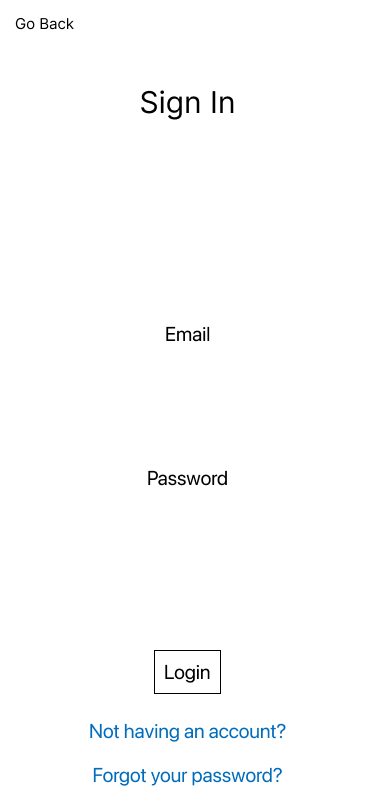
\includegraphics[width=0.3\linewidth]{figures/new-mockups/Login.png}}\label{fig:new-login}}
    \hfill
    \subfloat[Registration Screen]{\fbox{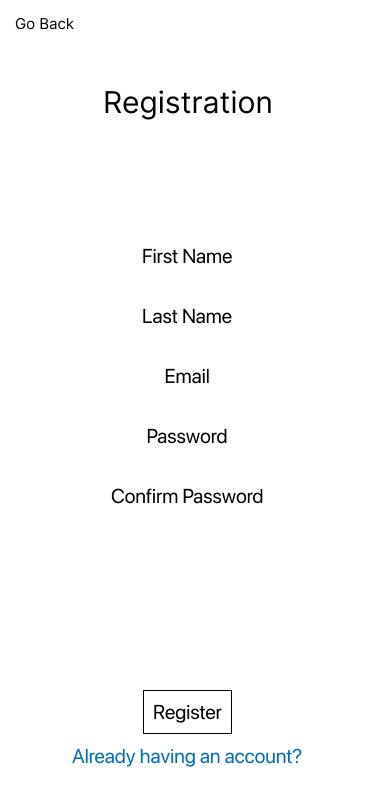
\includegraphics[width=0.3\linewidth]{figures/old-mockups/Registration.png}}\label{fig:new-registration}}
    \hfill
    \subfloat[Welcome Screen]{\fbox{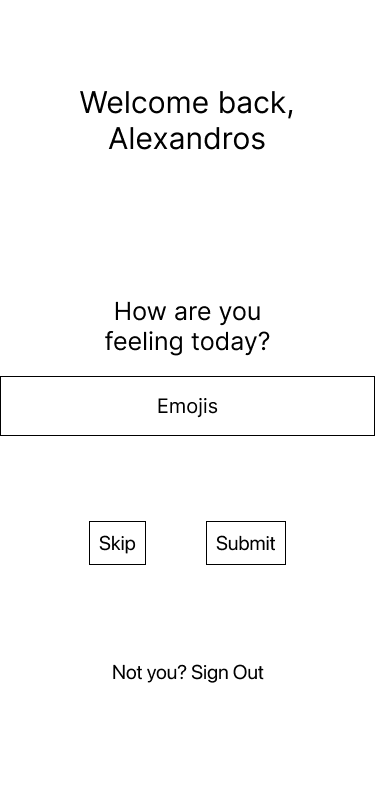
\includegraphics[width=0.3\linewidth]{figures/new-mockups/Welcome.png}}\label{fig:new-welcome}}
\end{figure}

\begin{figure}[htbp]\ContinuedFloat
    \centering
    \subfloat[Home Screen]{\fbox{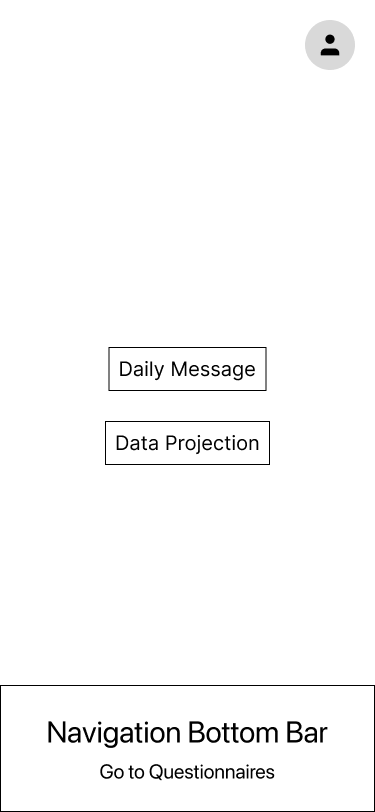
\includegraphics[width=0.3\linewidth]{figures/new-mockups/Home.png}}\label{fig:new-home}}
    \hfill
    \subfloat[Profile Screen]{\fbox{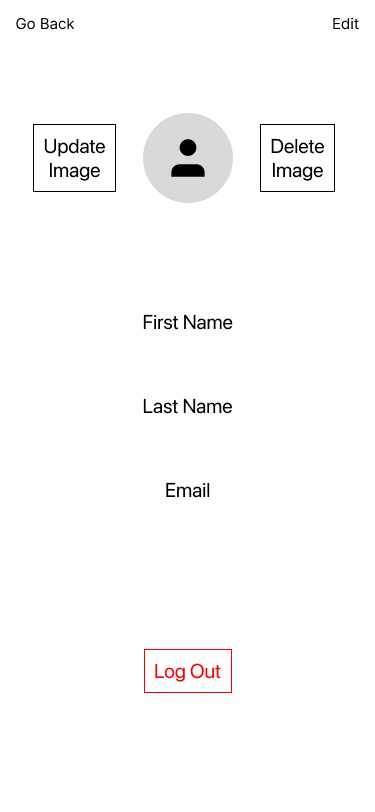
\includegraphics[width=0.3\linewidth]{figures/new-mockups/Profile.png}}\label{fig:new-profile}}
    \hfill
    \subfloat[Questionnaires Screen]{\fbox{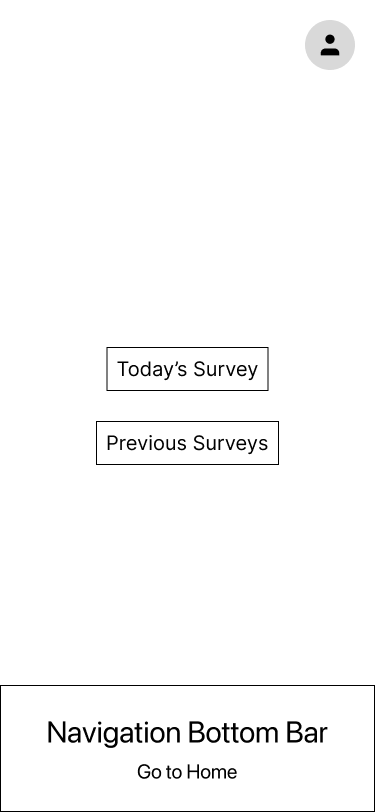
\includegraphics[width=0.3\linewidth]{figures/new-mockups/Questionnaires.png}}\label{fig:new-questionnaires}}
\end{figure}

\begin{figure}[htbp]\ContinuedFloat
    \centering
    \subfloat[Today's Survey (All Screens)]{\fbox{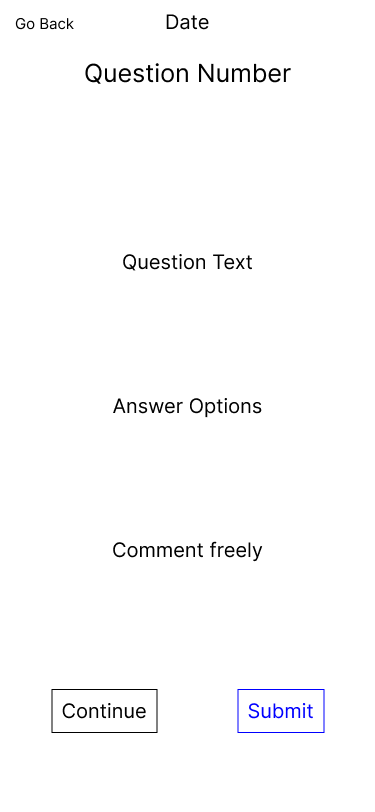
\includegraphics[width=0.3\linewidth]{figures/new-mockups/Today's Survey (All Pages).png}}\label{fig:new-todays_survey}}
    \hfill
    \subfloat[Previous Survey (All Screens)]{\fbox{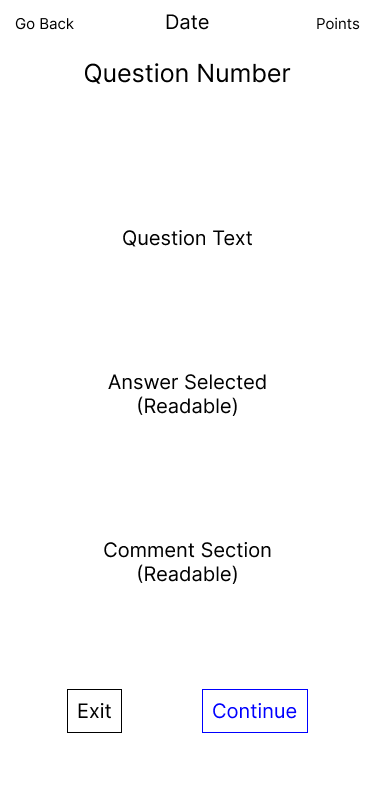
\includegraphics[width=0.3\linewidth]{figures/new-mockups/Previous Survey (All Pages).png}}\label{fig:new-previous_surveys}}
    \hfill
    \subfloat[Positive Confirmation Screen]{\fbox{
\includegraphics[width=0.3\linewidth]{figures/new-mockups/Positive Confirmation.png}}\label{fig:new-positive_confirmation}}
\end{figure}

\begin{figure}[htbp]\ContinuedFloat
    \centering
    \subfloat[Calendar Screen]{\fbox{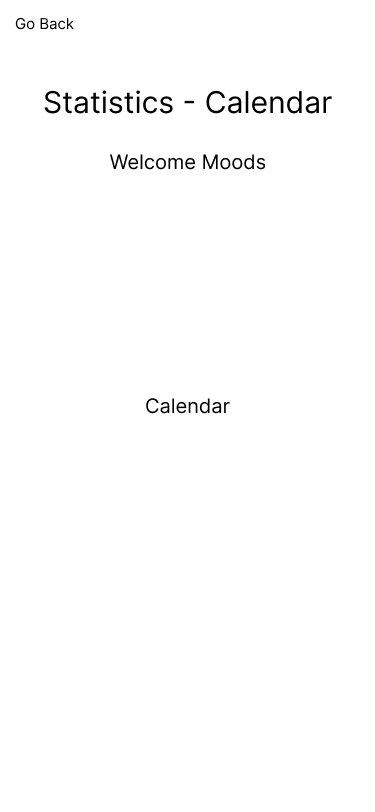
\includegraphics[width=0.3\linewidth]{figures/new-mockups/Calendar.png}}\label{fig:new-calendar}}
    \hfill
    \subfloat[Graph Screen]{\fbox{
\includegraphics[width=0.3\linewidth]{figures/new-mockups/Graph.png}}\label{fig:new-graph}}
\end{figure}

\begin{figure}[htbp]\ContinuedFloat
    \centering
    \subfloat[Request Password Reset Screen]{\fbox{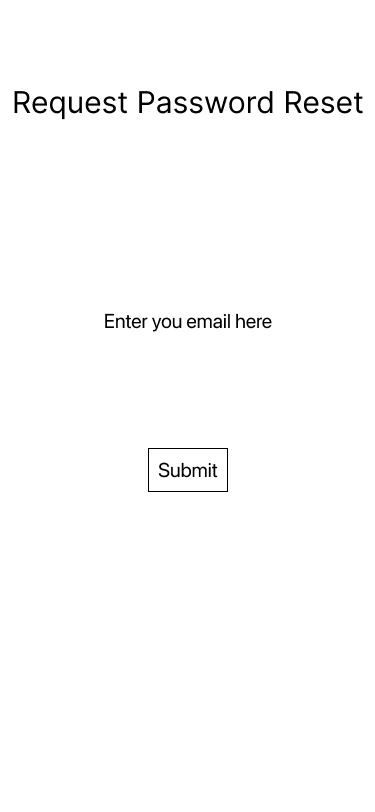
\includegraphics[width=0.3\linewidth]{figures/new-mockups/Request Password Reset.png}}\label{fig:request_password_reset}}
    \hfill
    \subfloat[Reset Password Screen]{\fbox{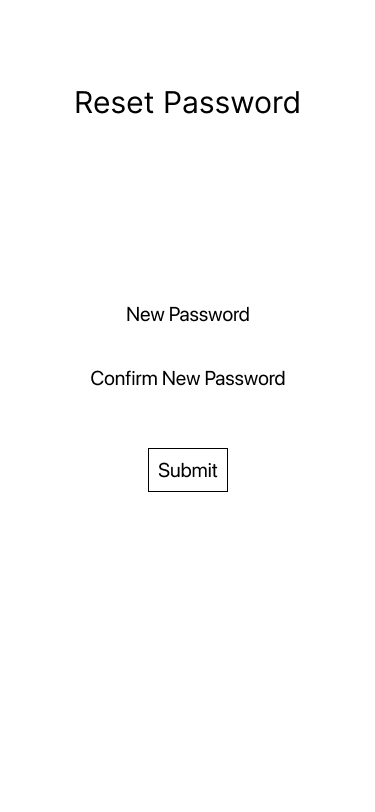
\includegraphics[width=0.3\linewidth]{figures/new-mockups/Reset Password.png}}\label{fig:reset_password}}
    \caption{(Updated) User Flow Screens}
    \label{fig:updated_user_flow_screens}
\end{figure}
\FloatBarrier

\section{Core Design Elements}

With the completion of all mockup screens, we turn our focus to defining the core design elements of the application, including colors, fonts, and icons. These design choices are based on the application research conducted in Chapter 2, alongside more in-depth personal research specific to each design aspect.

\subsection{Colors}

To design the color scheme for the application, we first conducted thorough research into color theory, principles, and best practices. The goal was to ensure that the selected colors would not only enhance the visual appeal but also align with the emotional tone and purpose of the app. This process involved exploring theoretical concepts, practical experimentation, and considerations for user interface design. \\

\noindent \textbf{Research and Resources} \\
To develop an effective color palette, a significant number of resources were used, like:

\begin{enumerate}
    \item \textbf{Adobe Documentation on Color Psychology \cite{adobe-color}} \\
    This documentation provided a comprehensive understanding of color meanings and symbolism. It explored how different colors evoke specific emotions and psychological responses, which helped in aligning the application's color choices with its purpose of mood tracking. The guide also offered tips on choosing brand colors that appeal to users and create a consistent design.
    \vspace{5mm}
    \item \textbf{YouTube Videos} \\
    A variety of useful YouTube videos were used to understand basic principles and serve as a valuable guide throughout the design process. Some of them are:

    \begin{itemize}
        \item \textbf{\href{https://www.youtube.com/watch?v=V-SD_zV9S2c}{The 60-30-10 Rule in Color Theory}} \\
        Link: \url{https://www.youtube.com/watch?v=V-SD_zV9S2c}
        \item \textbf{\href{https://www.youtube.com/watch?v=BdJTnYqhaZQ}{Brand Colors Selection}} \\
        Link: \url{https://www.youtube.com/watch?v=BdJTnYqhaZQ}
        \item \textbf{\href{https://www.youtube.com/watch?v=F-Zw7CbM-ps}{Logo Color Selection}} \\
        Link: \url{https://www.youtube.com/watch?v=F-Zw7CbM-ps}
        \item \textbf{\href{https://www.youtube.com/watch?v=u5AnzLg1HxY}{Design Color Palettes}} \\
        Link: \url{https://www.youtube.com/watch?v=u5AnzLg1HxY}
        \item \textbf{\href{https://www.youtube.com/watch?v=eXcKOqviLE0}{Apply Color Palette to Design}} \\
        Link: \url{https://www.youtube.com/watch?v=eXcKOqviLE0}
    \end{itemize}    

    \noindent The YouTube videos provided valuable insights into various aspects of color theory and its practical application in design. The 60-30-10 rule helped in understanding how to balance primary (brand), secondary, and accent colors to create visually appealing and balanced designs. Videos on brand and logo color selection emphasized the importance of choosing colors that reflect the application's identity and purpose. Additionally, tutorials on creating and applying color palettes to design ensured a deeper understanding of how to build appealing palettes that work well together across different elements, while maintaining readability and accessibility. These resources helped me create some possible color palettes for the application, so we can test and evaluate each of them.
\end{enumerate}

\vspace{5mm}

\noindent \textbf{Color Testing and Tools} \\
Once a solid theoretical foundation is established, we can test the potential color schemes using \textbf{Figma}, experimenting with brand, secondary, and accent colors. The goal was to identify color combinations that worked harmoniously together while ensuring readability and accessibility across various backgrounds. To further refine our choices, we employed several online tools:

\begin{itemize}
    \item \textbf{\href{https://color.adobe.com/create/color-wheel}{Adobe Color Wheel}}: A tool for experimenting with different color harmonies and combinations. \\
    Link: \url{https://color.adobe.com/create/color-wheel}
    \item \textbf{\href{https://huemint.com/}{Huemint}}: Useful for visualizing how the selected colors would appear on a website platform. \\
    Link: \url{https://huemint.com/}
    \item \textbf{\href{https://coolors.co/}{Coolors}}: Helpful for generating strong color palettes. \\
    Link: \url{https://coolors.co/}
    \item \textbf{\href{https://colorhunt.co/}{Color Hunt}}: Provided access to well-tested color palettes, helping us refine our choices. \\
    Link: \url{https://colorhunt.co/}
\end{itemize}


\vspace{5mm}

\noindent \textbf{Final Color Choices} \\
Using these valuable tools, we decided that the application should use shades of blue and shades of green as its brand colors. Blue is chosen as the primary color, expressing calmness, trust, and reliability, while green serves as the accent color, representing growth, balance, and positivity.\vspace{5mm} \\
Drawing inspiration from previous applications, particularly for the emoji selector, we selected specific colors to represent the different moods in the ``Welcome Mood'' emojis. The colors for the five emojis are:

\begin{itemize}
    \item \textbf{Awful}: A shade of dark red, symbolizing intense negative emotions.
    \item \textbf{Sad}: A blend of red and orange, reflecting a muted sense of distress.
    \item \textbf{Neutral}: A shade of yellow, representing balance and neutrality.
    \item \textbf{Good}: A vibrant shade of green, denoting positive emotions.
    \item \textbf{Happy}: A light and calming shade of blue, expressing happiness and positivity.
\end{itemize}

\noindent For text and other interface elements, the shades of blue and green are applied appropriately to maintain visual consistency and alignment with the application's tone.\vspace{5mm} \\
Additionally, basic colors such as white, black, and shades of gray are used throughout the design. White offers a clean and simple background, enhancing readability, while black provides contrast for text and important elements. The various shades of gray are employed for neutral backgrounds and subtle distinctions between UI components. As mentioned in the resources, using neutral tones like gray, black, and white helps maintain balance in the color scheme, ensuring that the brand colors and accents stand out without overwhelming the user interface.

\vspace{5mm}

\noindent \textbf{Shading} \\
After selecting the core colors for the application, we employed a technique from one of the referenced YouTube videos, along with the \textbf{\href{https://maketintsandshades.com/}{Tint and Shade Generator}}\footnote{Link: \url{https://maketintsandshades.com/}} tool, to generate various shades of the selected colors. The purpose of these shades is to provide a more versatile and united color scheme throughout the application.\vspace{5mm} \\
To create a consistent and balanced interface, nine different shades were generated for each primary and accent color. This approach ensures that we have lighter and darker variations of each color, which can be used for:
\begin{itemize}
    \item \textbf{Lighter shades}: For backgrounds, highlighting, or less dominant elements.
    \item \textbf{Darker shades}: For text, buttons, or to emphasize important components.
\end{itemize}
\noindent Of course, this also applies vice versa, like using darker shades for the background of a screen and lighter shades for the text of it.\vspace{5mm} \\
The technique used to create the shades ensures consistency across different colors, allowing the shades of various colors to maintain a similar visual structure. This approach stabilizes the design, meaning that if a blue shade is swapped with a green shade in the future, the overall interface retains its united look and feel. By ordering the shades properly, the application remains visually consistent, even when colors changes.\vspace{5mm} \\
Below the final color palette is shown, so we can notice the consistency of the shades when switching between the colors:

\vspace{5mm}

\FloatBarrier
\begin{table}[ht]
\centering
\begingroup
\setlength{\tabcolsep}{10pt}
\renewcommand{\arraystretch}{1.5}
\begin{tabular}{|c|p{1.5cm}<{\centering}|p{1.5cm}<{\centering}|p{1.5cm}<{\centering}|p{1.5cm}<{\centering}|p{1.5cm}<{\centering}|p{1.5cm}<{\centering}|}
\hline
\textbf{Shade} & \textbf{Blue} & \textbf{Green} & \textbf{Red} & \textbf{Orange} & \textbf{Yellow} & \textbf{Gray} \\ \hline
100 & \colorbox{blue100}{\strut \ \ \ \ \ \ } & \colorbox{green100}{\strut \ \ \ \ \ \ } & \colorbox{red100}{\strut \ \ \ \ \ \ } & \colorbox{orange100}{\strut \ \ \ \ \ \ } & \colorbox{yellow100}{\strut \ \ \ \ \ \ } & \colorbox{gray100}{\strut \ \ \ \ \ \ } \\
200 & \colorbox{blue200}{\strut \ \ \ \ \ \ } & \colorbox{green200}{\strut \ \ \ \ \ \ } & \colorbox{red200}{\strut \ \ \ \ \ \ } & \colorbox{orange200}{\strut \ \ \ \ \ \ } & \colorbox{yellow200}{\strut \ \ \ \ \ \ } & \colorbox{gray200}{\strut \ \ \ \ \ \ } \\
300 & \colorbox{blue300}{\strut \ \ \ \ \ \ } & \colorbox{green300}{\strut \ \ \ \ \ \ } & \colorbox{red300}{\strut \ \ \ \ \ \ } & \colorbox{orange300}{\strut \ \ \ \ \ \ } & \colorbox{yellow300}{\strut \ \ \ \ \ \ } & \colorbox{gray300}{\strut \ \ \ \ \ \ } \\
400 & \colorbox{blue400}{\strut \ \ \ \ \ \ } & \colorbox{green400}{\strut \ \ \ \ \ \ } & \colorbox{red400}{\strut \ \ \ \ \ \ } & \colorbox{orange400}{\strut \ \ \ \ \ \ } & \colorbox{yellow400}{\strut \ \ \ \ \ \ } & \colorbox{gray400}{\strut \ \ \ \ \ \ } \\
500 & \colorbox{blue500}{\strut \ \ \ \ \ \ } & \colorbox{green500}{\strut \ \ \ \ \ \ } & \colorbox{red500}{\strut \ \ \ \ \ \ } & \colorbox{orange500}{\strut \ \ \ \ \ \ } & \colorbox{yellow500}{\strut \ \ \ \ \ \ } & \colorbox{gray500}{\strut \ \ \ \ \ \ } \\
600 & \colorbox{blue600}{\strut \ \ \ \ \ \ } & \colorbox{green600}{\strut \ \ \ \ \ \ } & \colorbox{red600}{\strut \ \ \ \ \ \ } & \colorbox{orange600}{\strut \ \ \ \ \ \ } & \colorbox{yellow600}{\strut \ \ \ \ \ \ } & \colorbox{gray600}{\strut \ \ \ \ \ \ } \\
700 & \colorbox{blue700}{\strut \ \ \ \ \ \ } & \colorbox{green700}{\strut \ \ \ \ \ \ } & \colorbox{red700}{\strut \ \ \ \ \ \ } & \colorbox{orange700}{\strut \ \ \ \ \ \ } & \colorbox{yellow700}{\strut \ \ \ \ \ \ } & \colorbox{gray700}{\strut \ \ \ \ \ \ } \\
800 & \colorbox{blue800}{\strut \ \ \ \ \ \ } & \colorbox{green800}{\strut \ \ \ \ \ \ } & \colorbox{red800}{\strut \ \ \ \ \ \ } & \colorbox{orange800}{\strut \ \ \ \ \ \ } & \colorbox{yellow800}{\strut \ \ \ \ \ \ } & \colorbox{gray800}{\strut \ \ \ \ \ \ } \\
900 & \colorbox{blue900}{\strut \ \ \ \ \ \ } & \colorbox{green900}{\strut \ \ \ \ \ \ } & \colorbox{red900}{\strut \ \ \ \ \ \ } & \colorbox{orange900}{\strut \ \ \ \ \ \ } & \colorbox{yellow900}{\strut \ \ \ \ \ \ } & \colorbox{gray900}{\strut \ \ \ \ \ \ } \\ \hline
\end{tabular}
\endgroup
\caption{Final Color Palette}
\label{tab:final_color_palette}
\end{table}
\FloatBarrier

\noindent Finally, we added two levels of transparency (alpha levels) for the primary colors (blue, green, gray, etc.). These transparent variations (alpha=0.7 and alpha=0.5) are particularly useful when smoother transitions between colors are needed in the application, creating a more smooth and satisfying user experience. The transparent colors allow elements like overlays, backgrounds, or hover effects to blend seamlessly with the rest of the design.

\subsection{Fonts}
For the font selection, I wanted to find a modern, pleasant font that complements the overall character of the application. After careful consideration, I chose the ``Outfit'' font for its smooth curves and ``up to date feel'', making it a natural fit for the app’s interface. Multiple variations of ``Outfit'' are included (Regular, Medium, Bold) to provide flexibility for different text elements within the app.\vspace{5mm} \\
Additionally, I included the ``Roboto'' font, which is widely supported on both iOS and Android. This ensures that in case the primary fonts fail to load during the development or usage, the app maintains readability and consistency across platforms. The ``FjallaOne'' font is used in specific cases where a slimmer, sleeker look is desired for the text.\vspace{5mm} \\
Lastly, the ``Press Start 2P'' font, famously used in Google’s dinosaur game when the internet connection is down, has been included for a specific animation within the app. This choice allows for a fun feel that mimics the Google animation’s style.\vspace{5mm} \\
The fonts that we are going to work with in the developement phase, are as follows:
\begin{itemize}
    \item \textbf{Outfit}:
    \begin{itemize}
        \item Regular (Outfit-Regular.ttf)
        \item Medium (Outfit-Medium.ttf)
        \item Bold (Outfit-Bold.ttf)
    \end{itemize}
    \item \textbf{Roboto}:
    \begin{itemize}
        \item Regular (Roboto-Regular.ttf)
        \item Italic (Roboto-Italic.ttf)
        \item Medium (Roboto-Medium.ttf)
        \item Medium Italic (Roboto-MediumItalic.ttf)
        \item Bold (Roboto-Bold.ttf)
        \item Bold Italic (Roboto-BoldItalic.ttf)
    \end{itemize}
    \item \textbf{FjallaOne}:
\begin{itemize} \item Regular (FjallaOne-Regular.ttf) \end{itemize}
    \item \textbf{Press Start 2P}:
\begin{itemize} \item Regular (PressStart2P-Regular.ttf) \end{itemize}
\end{itemize}

\subsection{Icons}

For the icons that are going to be used in the application, I initially searched for SVG files, some of which I found online or created myself. However, after discovering that Expo offers a comprehensive library of vector icons (available at \textbf{\href{https://icons.expo.fyi/Index}{Expo Vector Icons}}\footnote{Link: \url{https://icons.expo.fyi/Index}}), I decided to rely on this resource. Expo Vector Icons provide a wide variety of scalable, customizable icons that flawless merge with the application.\vspace{5mm} \\
In the app's development, I am using these icons for key navigation elements, such as the ``Home Screen'' and the ``Questionnaires Screen'' in the bottom navigation bar. Additional icons are also selected from the Expo library for smaller features and functionalities.\vspace{5mm} \\
The icons used for the ``Welcome Mood'' on the ``Welcome Screen'' and ``Calendar Screen'' are as follows:

\FloatBarrier
\begin{figure}[htbp]
    \centering
    \subfloat[Nothing]{
\includegraphics[width=0.1\linewidth]{figures/icons/nothing.png}}
    \label{fig:welcome-mood-nothing}
    \hfill
    \subfloat[Awful]{
\includegraphics[width=0.1\linewidth]{figures/icons/awful.png}}
    \label{fig:welcome-mood-awful}
    \hfill
    \subfloat[Sad]{
\includegraphics[width=0.1\linewidth]{figures/icons/sad.png}}
    \label{fig:welcome-mood-sad}
    \hfill
    \subfloat[Neutral]{
\includegraphics[width=0.1\linewidth]{figures/icons/neutral.png}}
    \label{fig:welcome-mood-neutral}
    \hfill
    \subfloat[Good]{
\includegraphics[width=0.1\linewidth]{figures/icons/good.png}}
    \label{fig:welcome-mood-good}
    \hfill
    \subfloat[Happy]{
\includegraphics[width=0.1\linewidth]{figures/icons/happy.png}}
    \label{fig:welcome-mood-happy}
    \caption{Welcome Moods}
\end{figure}
\FloatBarrier

\noindent The ``Nothing'' emoji is used in instances when the user chooses not to respond or does not want to select a specific emoji for their mood. This option ensures that the user does not feel pressured to choose a mood if they are undecided or wish to skip the step without providing a specific input.\vspace{5mm} \\
The other five icons - ``Awful'', ``Sad'', ``Neutral'', ``Good'', and ``Happy'' – are easy to understand and provide clear differences in emotional states, visually representing a spectrum from negative to positive feelings. These icons are designed to capture a climactic progression, ensuring that each ``Welcome Mood'' is distinct and projects an easily recognizable emotional difference. This not only helps the user identify their feelings more clearly, but also makes it easier to visualize mood trends over time when projected in the ``Calendar Screen''.\vspace{5mm} \\
Furthermore, these moods perfectly align with the core question ``How are you feeling today?'', that is been shown in the ``Welcome Screen''. Each icon serves to provide a quick and natural response, encouraging user engagement while also ensuring the process of logging daily moods remains simple and meaningful.

\subsection{Animations}

For the application’s animations, I thought of using SVG files, but as mentioned in the Icons subsection, they make the implementation more difficult. Based on this, I plan to use pre-made Lottie animations from \textbf{\href{https://lottiefiles.com/}{LottieFiles}}\footnote{Link: \url{https://lottiefiles.com/}}. These animations are not only visually pleasing but also easy to implement, and they come in two formats: small animations and full-screen animations (such as splash screens). I intend to use them on the welcome screen to create a warm, engaging experience for users when they first open the app.\vspace{5mm} \\
Additionally, Lottie animations are embodied to signal the completion of surveys, increase user satisfaction. They are also used for the loading screen and the main splash screen of the application, giving it a polished and dynamic feel. Lastly, I plan to integrate these animations into any features that involve completion, loading, or other processes that require some time to complete, providing users with a smooth and visually engaging experience throughout the app.

\section{Inspiration for Design}

For inspiration when designing the screens and components of the application, I was inspired by the research conducted on other mood tracking apps, as discussed in Chapter 2. However, a significant portion of my design inspiration came from \textbf{\href{https://dribbble.com/following}{Dribbble}}\footnote{Link: \url{https://dribbble.com/following}}, a platform that promotes work by designers and developers from around the world. Dribbble is a hub for creativity where professionals share their designs for various digital products, including mobile apps, websites, and user interfaces.\vspace{5mm} \\
What makes Dribbble particularly useful is its search functionality, allowing users to explore an extensive library of visual ideas across a variety of categories. While the site primarily serves as a portfolio platform for designers who offer their services for hire, it also provides an excellent source of inspiration. By browsing through design concepts, even though they are available only as static images without code, you can gain valuable insights into layout, color schemes, and interaction ideas.\vspace{5mm} \\
Using Dribbble, I was able to gather inspiration for key components and screens that I plan to implement in my application. As we proceed further down, I describe the specific screens and components that were affected by this research.

\subsection{Screens}

\noindent \textbf{Profile} \\
For the Profile screen, I was inspired by the sleek and modern design of input fields. The simple and smooth combination of colors between the fields and the background creates a clean and organized look. I particularly liked how the information is displayed in editable text input fields, allowing users to quickly make changes by pressing the ``Done'' button at the top right. Additionally, I appreciate the layout of the avatar image, positioned above the fields, leaving space (left and right) for potential action buttons, such as ``Update'' or ``Delete'' for profile image modifications.

\vspace{5mm}

\FloatBarrier
\begin{figure}[htbp]
    \centering
    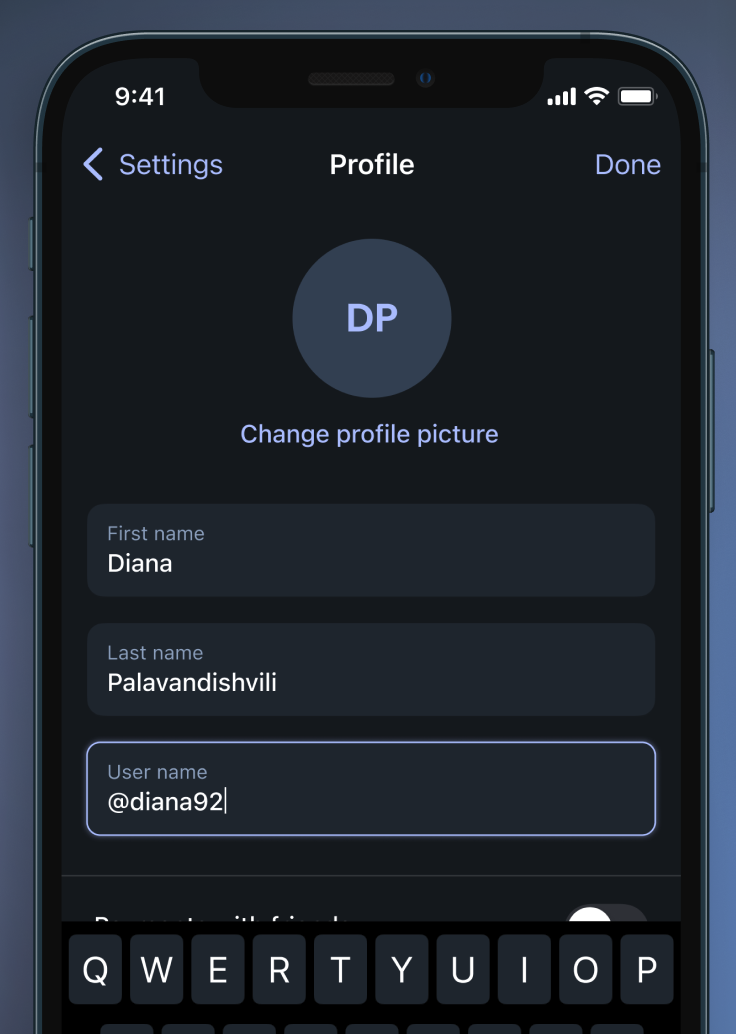
\includegraphics[width=0.5\linewidth]{figures/inspiration/Profile.png}
    \caption{Profile Screen}
    \label{fig:profile_inspiration}
\end{figure}
\FloatBarrier

\vspace{5mm}

\noindent \textbf{Home} \\
The Home screen design is visually appealing and well-organized. I am particularly drawn to the layout, which divides the content into three distinct sections. Each section holds relevant information in a clean, readable format. The navigation bar at the bottom is especially well designed, and I intend to incorporate this concept into my application to ensure a smooth and intuitive user experience.

\vspace{5mm}

\FloatBarrier
\begin{figure}[htbp]
    \centering
    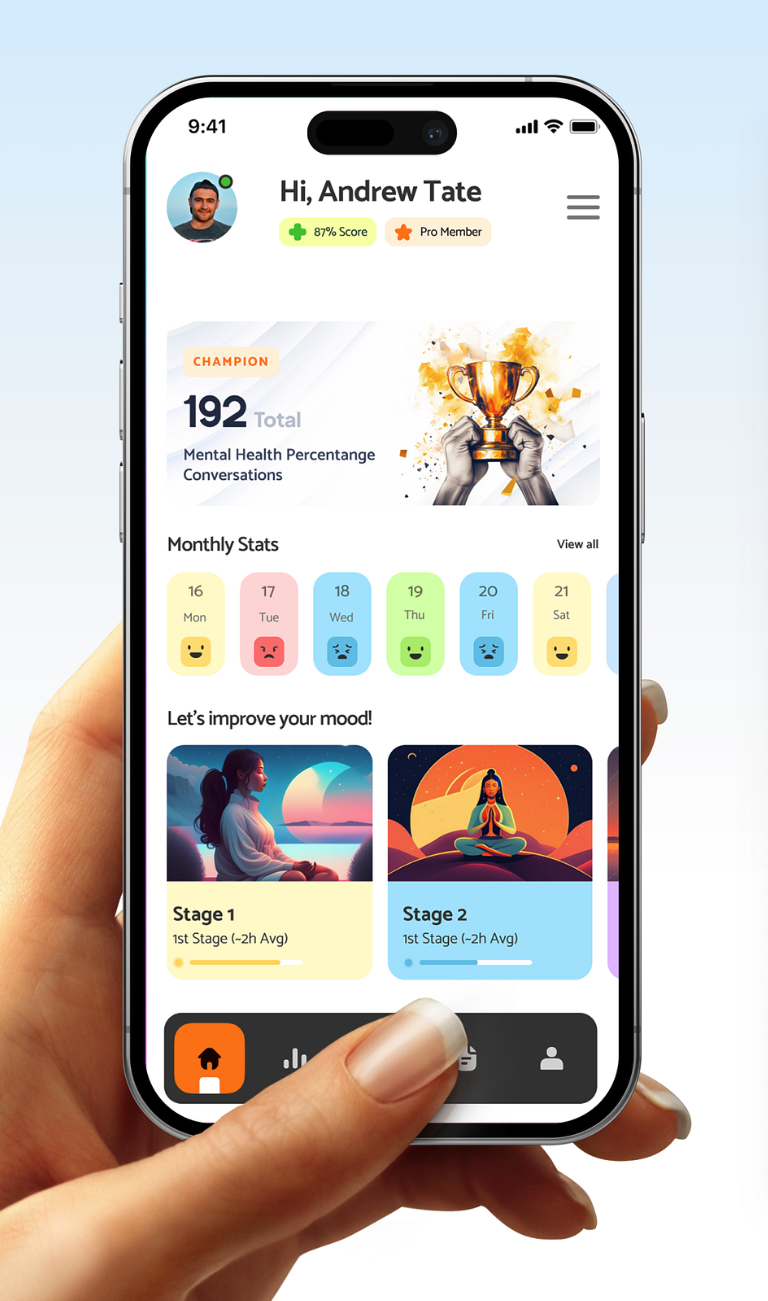
\includegraphics[width=0.45\linewidth]{figures/inspiration/Home.png}
    \caption{Home Screen}
    \label{fig:home_inspiration}
\end{figure}
\FloatBarrier

\subsection{Components}

\noindent \textbf{Calendar} \\
For the calendar component in the ``Calendar Screen'', I found two compelling designs that both use emojis to represent user moods. I plan to implement a similar concept for tracking the user’s ``Welcome Moods'' in my application. This allows for better visualization of the user's emotional data in a clear and straightforward manner, displaying only the most important infromation, the mood, the date, and the month-year format. The calendar features the same emojis that users select on the Welcome screen, ensuring consistency across the app.

\vspace{5mm}

\FloatBarrier
\begin{figure}[htbp]
    \centering
    \subfloat[Option 1]{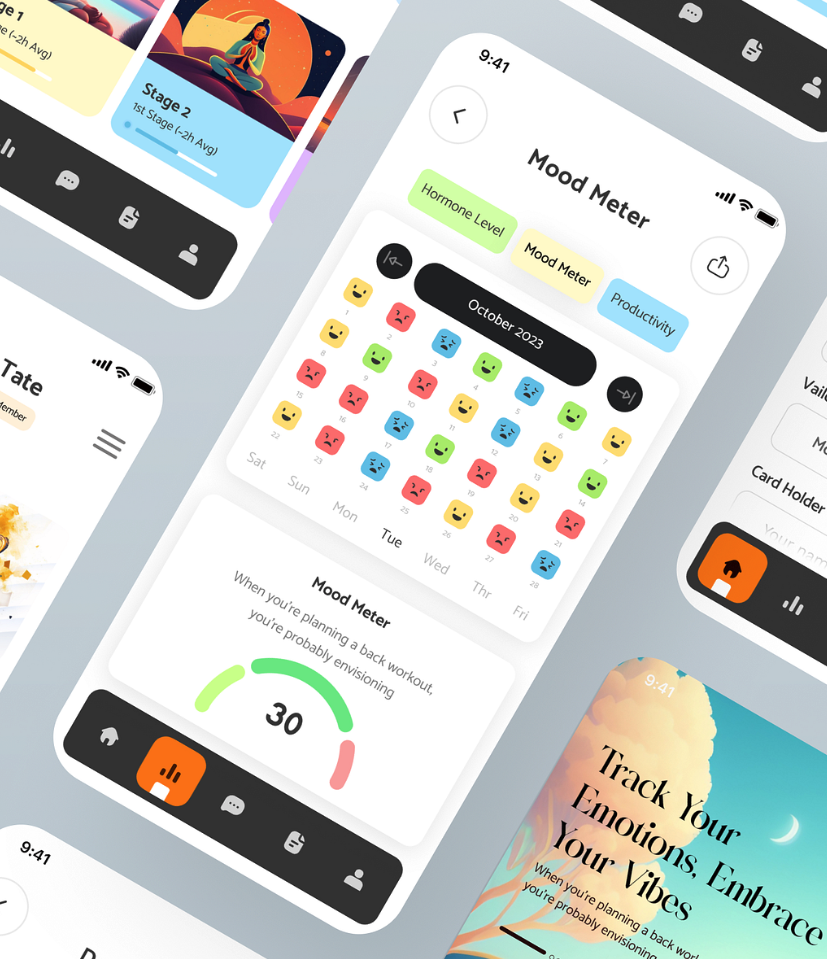
\includegraphics[width=0.49\linewidth]{figures/inspiration/Mood Calendar - 1.png}}\label{fig:mood_calendar_1}
    \hfill
    \subfloat[Option 2]{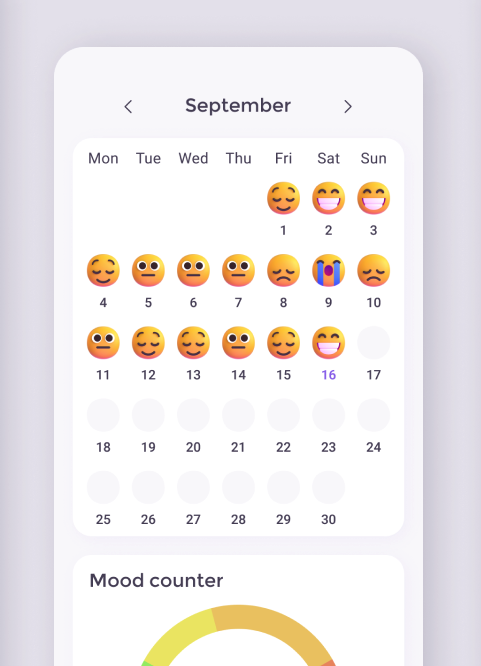
\includegraphics[width=0.41\linewidth]{figures/inspiration/Mood Calendar - 2.png}}\label{fig:mood_calendar_2}
    \caption{Mood Calendar Options}
\end{figure}
\FloatBarrier

\vspace{5mm}

\noindent \textbf{Graph} \\
When it comes to displaying data in the form of graphs in the ``Graph Screen'', I found two bar chart designs that I find both simple and effective. The idea is to show the user's survey results using vertical bars, with different colors representing varying scores. This makes it easier for users to quickly explain their performance without having to analyze complex data. I plan to use different colors to indicate low, average, and high scores for the completed questionnaires.

\vspace{5mm}

\FloatBarrier
\begin{figure}[htbp]
    \centering
    \subfloat[Option 1]{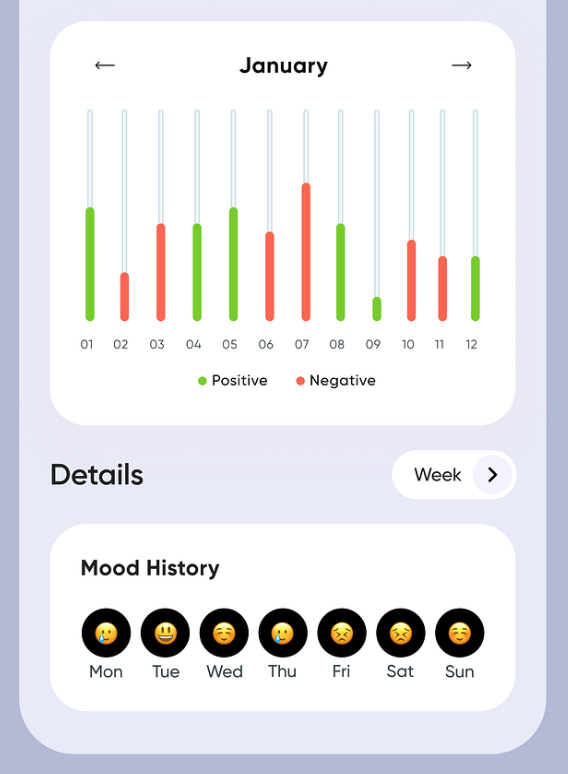
\includegraphics[width=0.48\linewidth]{figures/inspiration/Bar Chart - 1.png}}\label{fig:bar_chart_1}
    \hfill
    \subfloat[Option 2]{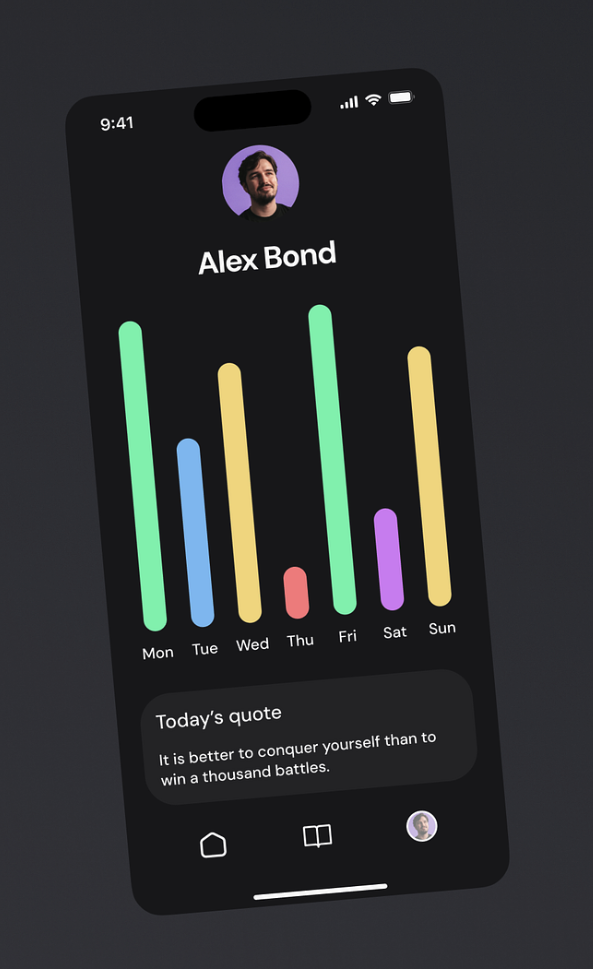
\includegraphics[width=0.4\linewidth]{figures/inspiration/Bar Chart - 2.png}}\label{fig:bar_chart_2}
    \caption{Bar Chart Options}
\end{figure}
\FloatBarrier

\vspace{5mm}

\noindent \textbf{Weekly Stats} \\
The Monthly Stats component from the picture [\ref{fig:weekly_stats}], which is featured as Weekly Stats on the Home screen of the applciation, provides a compact yet informative overview of the user’s mood data. This design, inspired by the Home screen layout, is scrollable and contains only the most essential details, making it easy to navigate and comprehend. This small version of the calendar data gives users a quick snapshot of their mood history.

\vspace{5mm}

\FloatBarrier
\begin{figure}[htbp]
    \centering
    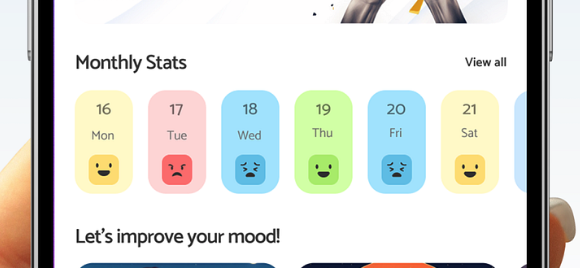
\includegraphics[width=0.5\linewidth]{figures/inspiration/Weekly Stats.png}
    \caption{Weekly Stats}
    \label{fig:weekly_stats}
\end{figure}
\FloatBarrier

\vspace{5mm}

\noindent \textbf{Header} \\
For the header component, I was inspired from a design that incorporates a friendly, personalized greeting, such as ``Hello, \{User Name\}''. This adds a personal touch to the user’s experience. Below the greeting, the application displays additional information, but instead of showing a health score or pro member status (as seen in the example [\ref{fig:header}], I plan to include the user’s streak and an icon indicating whether they have completed that day's survey. The avatar is placed on the right side, and pressing it can navigate users to the Profile screen.

\vspace{5mm}

\FloatBarrier
\begin{figure}[htbp]
    \centering
    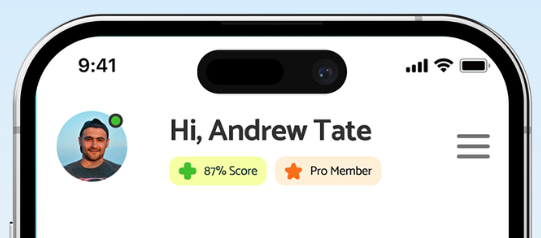
\includegraphics[width=0.45\linewidth]{figures/inspiration/Header.png}
    \caption{Header}
    \label{fig:header}
\end{figure}
\FloatBarrier

\section{Summary}

In this chapter, we focused on designing an application that is not only functional but also visually appealing and user-friendly. By developing a clear structure and incorporating elements such as colors, fonts, icons, and animations, we aimed to create an interface that is both engaging and easy to navigate. The choice of design elements is crucial for fostering a sense of safety and trust among users, encouraging them to use the application consistently. This foundation will support students in feeling comfortable and secure while interacting with the app. In the next chapter, we turn our attention to the technical implementation, bringing the design concepts and research insights into reality.